%!TEX TS-program = xelatex
% https://habr.com/ru/post/144648/
\documentclass[a4paper,14pt,ukrainian]{extreport}
\usepackage{xltxtra}

\usepackage{extsizes}
%\usepackage{cmap} % для кодировки шрифтов в pdf
\usepackage{fontspec}
\defaultfontfeatures{Ligatures={TeX}} 
\setmainfont[Ligatures=TeX]{Times New Roman}
\setmonofont[Mapping=tex-text]{Courier New}
\usepackage[ukrainian]{babel}

\usepackage{graphicx} % для вставки картинок
\usepackage{amssymb,amsfonts,amsmath,amsthm} % математические дополнения от АМС
\usepackage{indentfirst} % отделять первую строку раздела абзацным отступом тоже
\usepackage[usenames,dvipsnames]{color} % названия цветов
\usepackage{makecell}
\usepackage{multirow} % улучшенное форматирование таблиц
\usepackage{ulem} % подчеркивания

\usepackage{tikz}
\usepackage{pgfplots}
\pgfplotsset{compat=1.17}
\usepackage[europeanresistors, RPvoltages]{circuitikz}
\usetikzlibrary{arrows,decorations.markings}

\usepackage[nodisplayskipstretch]{setspace}
\onehalfspacing % полуторный интервал
\frenchspacing

\usepackage{fancyhdr}
\pagestyle{fancy}
\fancyhf{}
\fancyhead[R]{\thepage}
\fancyheadoffset{0mm}
\fancyfootoffset{0mm}
\setlength{\headheight}{17pt}
\renewcommand{\headrulewidth}{0pt}
\renewcommand{\footrulewidth}{0pt}
\fancypagestyle{plain}{ 
    \fancyhf{}
    \rhead{\thepage}}
\setcounter{page}{1} 

\usepackage[tableposition=top]{caption}
\usepackage{subcaption}
\DeclareCaptionLabelFormat{gostfigure}{Рисунок #2}
\DeclareCaptionLabelFormat{gosttable}{Табл. #2}
\DeclareCaptionLabelSeparator{gost}{~--~}
\captionsetup{labelsep=gost}
\captionsetup[figure]{labelformat=gostfigure}
\captionsetup[table]{labelformat=gosttable}
\renewcommand{\thesubfigure}{\asbuk{subfigure}}

\usepackage{titlesec}
 
\titleformat{\chapter}[display]
    {\filcenter}
    {\bfseries\texorpdfstring{\MakeUppercase{\chaptertitlename}}{{\chaptertitlename}} \thechapter}
    {4pt}
    {\bfseries\MakeUppercase}{}
 
\titleformat{\section}
    {\normalsize\bfseries}
    {\thesection.}
    {1em}{}
 
\titleformat{\subsection}
    {\normalsize\bfseries}
    {\thesubsection.}
    {1em}{}

% Настройка вертикальных и горизонтальных отступов
\titlespacing*{\chapter}{0pt}{-30pt}{4pt}
\titlespacing*{\section}{\parindent}{*2}{*1}
\titlespacing*{\subsection}{\parindent}{*2}{*1}

\usepackage{geometry}
% \geometry{left=3cm}
% \geometry{right=1.5cm}
% \geometry{top=2.4cm}
% \geometry{bottom=2.4cm}
\geometry{left=2cm}
\geometry{right=1cm}
\geometry{top=2cm}
\geometry{bottom=2cm}

\usepackage{enumitem}
\makeatletter
    \AddEnumerateCounter{\asbuk}{\@asbuk}{м)}
\makeatother
\setlist{nolistsep}
%\renewcommand{\labelitemi}{-}
%\renewcommand{\labelenumi}{\asbuk{enumi})}
%\renewcommand{\labelenumii}{\arabic{enumii})}

\usepackage{tocloft}
\renewcommand{\cfttoctitlefont}{\hspace{0.38\textwidth} \bfseries\texorpdfstring{\MakeUppercase}{}}
\renewcommand{\cftbeforetoctitleskip}{-0.5em}
%\renewcommand{\cftaftertoctitle}{\mbox{}\hfill \\ \mbox{}\hfill{\footnotesize Стр.}\vspace{-2.5em}}
\renewcommand{\cftchapfont}{\normalsize \texorpdfstring{\MakeUppercase{\chaptername}}{{\chaptername}} }
\renewcommand\cftchappagefont{\mdseries}
\renewcommand{\cftsecfont}{\hspace{-11pt}}
\renewcommand{\cftsubsecfont}{\hspace{11pt}}
\renewcommand{\cftbeforechapskip}{1em}
\renewcommand{\cftparskip}{-1mm}
\renewcommand{\cftdotsep}{1}
\renewcommand{\cftchapleader}{\cftdotfill{\cftdotsep}}
\renewcommand{\cftsecaftersnum}{.}
\setcounter{tocdepth}{2} % задать глубину оглавления — до subsection включительно

\newcommand{\likechapterheading}[1]{ 
    \begin{center}
    \textbf{\texorpdfstring{\MakeUppercase{#1}}{{#1}}}
    \end{center}}

\makeatletter
    \newcommand{\l@likechapter}[2]{{\bfseries\@dottedtocline{0}{0pt}{0pt}{#1}{#2}}}
\makeatother
\newcommand{\likechapter}[1]{    
    \likechapterheading{#1}
    \phantomsection    
    \addcontentsline{toc}{likechapter}{\texorpdfstring{\MakeUppercase{#1}}{{#1}}}}

\usepackage[square,numbers,sort&compress]{natbib}
\renewcommand{\bibnumfmt}[1]{#1.\hfill} % нумерация источников в самом списке — через точку
\renewcommand{\bibsection}{\likechapter{Список використаної літератури}} % заголовок специального раздела
\setlength{\bibsep}{0pt}

\usepackage[hidelinks]{hyperref}
\usepackage{microtype}

\usepackage{listings}

\lstdefinestyle{code}{
    basicstyle=\ttfamily\footnotesize,
    breakatwhitespace=false,         
    breaklines=true,                 
    captionpos=b,                    
    keepspaces=true,                            
    numbersep=1pt,                  
    showspaces=false,                
    showstringspaces=false,
    showtabs=false,                  
    tabsize=2
}

\newcommand{\inlinecode}[1]{\texttt{\small #1}}

\usepackage{float}

\newcommand{\append}[1]{
    \phantomsection
    \addcontentsline{toc}{section}{#1}
    \begin{center}
        \textbf{#1}
    \end{center}
}

\begin{document}
\begin{titlepage}
    \thispagestyle{empty}
    \begin{center}
        Міністерство освіти і науки України\\
        Національний технічний університет України\\
        <<Київський політехнічний інститут ім. І. Сікорського>>\\
        Інститут прикладного системного аналізу
    \end{center}
    \vspace{50mm}
    \begin{center}
        \textbf{Курсова робота} \\
        з дисципліни \\
        <<Теорія керування>>
    \end{center}
    \vspace{30mm}
    \begin{flushright}
        \textbf{Виконав}: студент 4 курсу \\
        групи КА-81 \\
        Галганов Олексій \\
        \textbf{Прийняв}: професор \\
        Романенко Віктор Демидович
    \end{flushright}
    \vspace{40mm}
    \begin{center}
        \textbf{Київ 2021}
    \end{center}
\end{titlepage}
\microtypesetup{protrusion=false}
\tableofcontents
\microtypesetup{protrusion=true}
    % !TEX root = ../main.tex
\newpage
\chapter{Вступ}
\section{Теоретичні дані}
Розглядається одноконтурна система автоматичного цифрового керування (ЦК) з наступною структурною схемою:
\begin{figure}[!ht]
    \begin{circuitikz}[scale = 0.9, transform shape]
        \draw (0, 0) to[switch] (2, 0) node[above left = 0.3em]{$G(s)$} 
        to[lamp] (3, 0) to[switch] (5, 0) node[above left = 0.3em]{$E^*(s)$};
        \node[draw, minimum width = 2cm, minimum height = 1cm, anchor = south west] at (5, -0.5){$W_P^*(s)$};
        \draw (7, 0) to[switch] (9, 0) node[above left = 0.3em]{$u^*(s)$} (9, 0); 
        \node[draw, minimum width = 2cm, minimum height = 1cm, anchor = south west] at (9, -0.5){$W_E^*(s)$};
        \draw (11, 0) to (13, 0);
        \node at (12, 0.6) {$u(s)$};
        \node[draw, minimum width = 2cm, minimum height = 1cm, anchor = south west] at (13,-0.5){$W_O^*(s)$};
        \draw[decoration={markings,mark=at position 1 with
            {\arrow[scale=2,>=stealth]{>}}},postaction={decorate}] (15, 0) -- (17, 0);
        \draw[decoration={markings,mark=at position 1 with
            {\arrow[scale=2,>=stealth]{>}}},postaction={decorate}] (1.5, 0) -- (2.07, 0);
        \draw[decoration={markings,mark=at position 1 with
            {\arrow[scale=2,>=stealth]{>}}},postaction={decorate}] (4.5, 0) -- (5, 0);
        \draw[decoration={markings,mark=at position 1 with
            {\arrow[scale=2,>=stealth]{>}}},postaction={decorate}] (8.5, 0) -- (9, 0);
        \draw[decoration={markings,mark=at position 1 with
            {\arrow[scale=2,>=stealth]{>}}},postaction={decorate}] (12.5, 0) -- (13, 0);
        \draw[decoration={markings,mark=at position 1 with
            {\arrow[scale=2,>=stealth]{>}}},postaction={decorate}] (2.5, -2) -- (2.5, -0.4);
        \draw (2.5, -2) -- (10, -2);
        \draw (10, -2) to[switch] (12, -2) node[above left = 0.3em]{$y^*(s)$}; 
        \node [above = 0.3em] at (16, 0) {$y(s)$};
        \draw (12, -2) -- (16, -2) -- (16, 0);
        \node at (1.7, -0.4) {$+$};
        \node at (2.8, -0.8) {$-$};
        \draw [fill, radius=0.15em] (16, 0) circle;
    \end{circuitikz}
    \caption{Структурна схема типового контура ЦК}
    \label{pic1}
\end{figure}

Тут $W_O(s)$ -- передаточна функція об'єкта керування по керуючому діянню, $G(s)$ і $u(s)$ -- відповідно задаюче і керуюче діяння в формі
перетворення Лапласа, $W_p^*(s)$ -- передаточна функція цифрового регулятора (ЦАП) у формі дискретного перетворення Лапласа,
$W_E(s)$ -- передаточна функція цифро-аналогового регулятора, $E^*(s)$, $u^*(s)$, $y^*(s)$ -- відповідно помилка керування,
керуюче діяння та вихідна керована координата у формі дискретного перетворення Лапласа. Передаточні функції об'єкта для окремих задач мають вигляд
\begin{gather}\label{W_0}
    W_O(s) = \frac{
        k e^{-\tau s}
    }{
        (T_1 s + 1) (T_2 s + 1) (T_3 s + 1)
    } \\
    \label{W_0_12}
    W_O(s) = \frac{
        k (T_1 s + 1)
    }{
        (T_2 s + 1) (T_3 s + 1)
    }
\end{gather}
де $k$ -- коефіцієнт передачі об'єкта керування, $T_1$, $T_2$, $T_3$ -- сталі часу в секундах, $\tau$ -- час запізнення в секундах.

Регулятор ЦК, представлений в різницевій формі на основі позиційного алгоритма пропорційно-інтегрально-диференціального (ПІД)
закону керування записується таким чином:
\begin{gather}\label{PID}
    u(n T_0) = K_p \left(
        e(n T_0) + \frac{T_0}{T_I} \sum_{i=1}^n e(i T_0) +
        \frac{T_D}{T_0} \left[e(n T_0) - e((n-1)T_0)\right]
    \right)
\end{gather}
Тут $u(n T_0)$ та $e(n T_0)$ -- відповідно керуюче діяння і помилка керування в $n$-тий період квантування,
$K_p$ -- коефіцієнт передачі регулятора, $T_I$ та $T_D$ -- відповідно сталі часу інтегрування та диференціювання в секундах,
$T_0$ -- період квантування в секундах. 

Відповідно до \eqref{PID}, дискретна передаточна функція ПІД-регулятора має вигляд
\begin{gather}
    W_p(z) = K_p \left(
        1 + \frac{T_0}{T_I \left(1 - z^{-1}\right)} + \frac{T_D\left(1 - z^{-1}\right)}{T_0}
    \right)
\end{gather}
Якщо час диференціювання $T_D = 0$, то для цифрового ПІ-регулятора матимемо дискретну передаточну функцію
\begin{gather}\label{PI}
    W_p(z) = K_p \left(
        1 + \frac{T_0}{T_I \left(1 - z^{-1}\right)}
    \right)
\end{gather}
де $z = e^{sT_0}$ -- оператор $z$-перетворення.

\section{Завдання курсової роботи}
\begin{enumerate}
    \item Розрахувати дискретну передаточну функцію замкненого контура 
        цифрового керування, попередньо розрахувавши дискретну передаточну 
        функцію приведеної неперервної частини (ПНЧ) об'єкта
        \begin{gather}
            W_\text{п}(z) = z \left\{W_E(s) \cdot W_O(s) \right\}
        \end{gather} 
        для наступних варіантів передаточної функції об'єкта:
        $W_O(S) = \frac{k}{T_1 s + 1}$, $W_O(S) = \frac{k}{(T_1 s + 1)(T_2 s + 1)}$, 
        $W_O(S) = \frac{k e^{-\tau s}}{T_1 s + 1}$, $W_O(S) = \frac{k e^{-\tau s}}{(T_1 s + 1)(T_2 s + 1)}$.
    \item Розрахувати періоди квантування в системі цифрового керування для об'єктів
        \begin{gather}\label{W_01}
            W_{O_1}(s) = \frac{k e^{-\tau s}}{T_1 s + 1} \\
            \label{W_02}
            W_{O_2}(s) = \frac{k e^{-\tau s}}{(T_1 s + 1)(T_2 s + 1)}
        \end{gather}
        і для об'єкта \eqref{W_0_12}, передаточна функція якого має динаміку в чисельнику.
    \item На основі методу <<прямого>> синтезу визначити структуру і оптимальні настройки регуляторів цифрового керування і неперервного
        регулятора для управління об'єктами, передаточні функції яких мають вигляд \eqref{W_01}, \eqref{W_02}. 
        При цьому приймається період квантування $T_0$, розрахований у пункті 2 на основі умови забезпечення необхідної точності керування.
        Значення коефіцієнта підсилення регулятора
        $K_{P_\text{опт}}$ необхідно визначити при таких параметрах настройки $\lambda$:

        a) $\lambda = \frac{1}{T_1}$; б) $\lambda = \frac{1}{1.5 T_1}$; в) $\lambda = \frac{1}{2T_1}$; г) $\lambda = \frac{1}{3T_1}$.

        Для вказаного набору параметрів настройки $\lambda$ шляхом цифрового моделювання побудувати перехідні процеси в замкненому контурі цифрового керування.
    \item  Розрахувати оптимальні параметри ПІ-регулятора цифрового керування і 
        періоду квантування резонансним методом для об'єкта керування \eqref{W_0}, \eqref{W_02}. На основі цифрового моделювання побудувати перехідні процеси 
        вихідної координати $y$ в замкненому контурі при подачі імпульсних тестів 
        на задаюче діяння цифрового регулятора. 
    \item Виконати синтез лінійно-квадратичного регулятора стану і виконати 
        цифрове моделювання замкненої системи з регулятором стану. 
    \item Дослідити стійкість контура цифрового керування, розрахованої за 
        пунктом 3. При цьому використовувати відомі критерії стійкості. 
    \item Сформувати позиційний і швидкісний алгоритм цифрового керування в формі, зручній для програмування для регуляторів цифрового керування відповідно до пунктів 3, 4.
\end{enumerate}

\section{Значення коефіцієнтів та сталих}
\begin{center}
    \begin{tabular}{|c|c|c|c|c|}
        \hline
        $k$ & $T_1$ & $T_2$ & $T_3$ & $\tau$ \\
        \hline
        9.32 & 35 & 19 & 11 & 14 \\ 
        \hline
    \end{tabular}
\end{center}
$k$ -- коефіцієнт передачі об'єкта керування, $T_1$, $T_2$, $T_3$ -- сталі часу в секундах, $\tau$ -- час запізнення в секундах.
    \newpage
    % !TEX root = ../main.tex
\chapter{Розрахунок дискретних передаточних функцій}
\section{Теоретичні дані}
% Відповідно до рисунку \ref{pic1}, керовану координату $y(s)$
% можна записати як 
% \begin{gather}\label{eq:2_1}
%     y(s) = W_{n}(s) \cdot u^* (s)
% \end{gather}, де
% $u^*(s)$ -- дискретне перетворення Лапласа керуючого діяння $u(t)$,
% яке дорівнює
% \begin{gather}
%     u^*(s) = W_p^*(s) \cdot E^*(s)
% \end{gather}
% а $W_n(s) = W_E(s) \cdot W_O(S)$ -- передаточна функція приведеної неперервної частини.
% При цьому
% \begin{gather}
%     E^*(s) = G^*(s) - y^*(s) 
% \end{gather}
% де $E^*(s)$, $G^*(s)$, $y^*(s)$ --- відповідно дискретне перетворення Лапласа від
% помилки керування, задаючого діяння і керованої координати.

% Застосуємо до \eqref{eq:2_1} дискретне перетворення Лапласа:
% \begin{gather}
%     y^*(s) = W_{n}^*(s) \cdot u^*(s)
% \end{gather}
% Після

Дискретну передаточну функцію приведеної неперервної частини (ПНЧ)
об'єкта має вигляд
\begin{gather}
    \nonumber
    W_{\text{п}}(z) = z \left\{W_E(s) \cdot W_O(s) \right\} = 
    z\left\{ \frac{1-e^{-s T_0}}{s} \cdot W_O(S)\right\} = \\ =
    z\left\{\left(1 - e^{-s T_0}\right)\cdot \frac{W_O(s)}{s}\right\} = 
    \left(1 - z^{-1}\right) \cdot z\left\{\frac{W_O(s)}{s} \right\}
\end{gather}
Дискретна передаточна функція замкненого контуру цифрового керування має вигляд
\begin{gather}
    W_{\text{з}}(z) = \frac{
        W_{\text{п}}(z) \cdot W_p(z)
    }{1 + W_{\text{п}}(z) \cdot W_p(z)}
\end{gather}
де $W_p(z)$ -- дискретна передаточна функція регулятора, що для ПІД-регулятора
має вигляд \eqref{PID}, а для ПІ-регулятора -- вигляд \eqref{PI}.
Далі за текстом термін <<дискретна передаточна функція>> буде скорочено до ДПФ.

\section{Випадок \texorpdfstring{$W_O(S) = \frac{k}{T_1 s + 1}$}{1}}
Обчислимо $z$-перетворення для $\frac{W_O(S)}{s} = \frac{k}{s(T_1 s + 1)} = \frac{k}{s} - \frac{k T_1}{T_1 s + 1}$.
За таблицею $z$-перетворення отримаємо
\begin{gather}
    z\left\{\frac{W_O(s)}{s} \right\} = 
    \frac{kz}{z-1} - \frac{kz}{z - e^{T_0 / T_1}} = 
    \frac{k \left(1 - e^{- T_0 / T_1}\right)z}{
        (z-1) \left(z - e^{- T_0 / T_1}\right)
    }
\end{gather}
Тому ДПФ ПНЧ має вигляд
\begin{gather}
    W_{\text{п}}(z) = \left(1 - z^{-1}\right) \cdot z\left\{\frac{W_O(s)}{s} \right\} = 
    \frac{z-1}{z} \cdot \frac{k \left(1 - e^{- T_0 / T_1}\right)z}{
        (z-1) \left(z - e^{- T_0 / T_1}\right)
    } = \nonumber \\ =
    \frac{k \left(1 - e^{- T_0 / T_1}\right)}{
        z - e^{- T_0 / T_1}
    }
\end{gather}
Отже, ДПФ замкненого контуру цифрового керування з ПІД-регулятором має вигляд
\begin{gather}
    W_{\text{з}}(z) = \frac{
        W_{\text{п}} (z) \cdot W_p(z)
    }{1 + W_{\text{п}} (z) \cdot W_p(z)} = 
    \frac{
        \frac{k \left(1 - e^{- T_0 / T_1}\right)}{
            z - e^{- T_0 / T_1}
        } \cdot K_p \left(
            1 + \frac{T_0}{T_I \left(1 - z^{-1}\right)} + \frac{T_D\left(1 - z^{-1}\right)}{T_0}
        \right)
    }{
        1 + 
        \frac{k \left(1 - e^{- T_0 / T_1}\right)}{
            z - e^{- T_0 / T_1}
        } \cdot K_p \left(
            1 + \frac{T_0}{T_I \left(1 - z^{-1}\right)} + \frac{T_D\left(1 - z^{-1}\right)}{T_0}
        \right)
    } = \nonumber \\ =
    \frac{
        k \left(1 - e^{- T_0 / T_1}\right) \cdot K_p \left(
            1 + \frac{T_0}{T_I \left(1 - z^{-1}\right)} + \frac{T_D\left(1 - z^{-1}\right)}{T_0}
        \right)
    }{
        \left(z - e^{- T_0 / T_1}\right) + k \left(1 - e^{- T_0 / T_1}\right) \cdot K_p \left(
            1 + \frac{T_0}{T_I \left(1 - z^{-1}\right)} + \frac{T_D\left(1 - z^{-1}\right)}{T_0}
        \right)
    } = \nonumber \\ =
    \mbox{\normalsize $\frac{
        k K_p \left(1 - e^{- T_0 / T_1}\right)
        \left(
            T_0 T_I \left(1 - z^{-1}\right) + T_0^2 + T_I T_D \left(1 - z^{-1}\right)^2
        \right)
    }{
        \left(z - e^{- T_0 / T_1}\right) T_0 T_I \left(1 - z^{-1}\right) + k K_p \left(1 - e^{- T_0 / T_1}\right)
        \left(
            T_0 T_I \left(1 - z^{-1}\right) + T_0^2 + T_I T_D \left(1 - z^{-1}\right)^2
        \right) 
    }$} = \nonumber \\ =
    \mbox{\normalsize $\frac{
        k K_p \left(1 - e^{- T_0 / T_1}\right)
        \left(
            T_0 T_I \left(1 - z^{-1}\right) + T_0^2 + T_I T_D \left(1 - z^{-1}\right)^2
        \right) z^{-1}
    }{
        \left(1 - e^{- T_0 / T_1} z^{-1}\right) T_0 T_I \left(1 - z^{-1}\right) + k K_p \left(1 - e^{- T_0 / T_1}\right)
        \left(
            T_0 T_I \left(1 - z^{-1}\right) + T_0^2 + T_I T_D \left(1 - z^{-1}\right)^2
        \right) z^{-1}
    }$}
    % = \nonumber \\ =
    % \mbox{\normalsize $\frac{
    %     k K_p \left(z - e^{- T_0 / T_1}\right)
    %     \left(
    %         T_0 T_I  z \left(z - 1\right) + z^2 T_0^2 + T_I T_D \left(z - 1\right)^2
    %     \right)
    % }{
    %     \left(z - e^{- T_0 / T_1}\right) T_0 T_I z \left(z - 1\right) + k K_p \left(z - e^{- T_0 / T_1}\right)
    %     \left(
    %         T_0 T_I z \left(z - 1\right) + z^2 T_0^2 + T_I T_D \left(z - 1\right)^2
    %     \right)
    % }$}
\end{gather}
Відповідно, з ПІ-регулятором ($T_D = 0$):
\begin{gather}
    W_{\text{з}}(z) = \mbox{\normalsize $\frac{
        k K_p \left(1 - e^{- T_0 / T_1}\right)
        \left(
            T_0 T_1 \left(1 - z^{-1}\right) + T_0^2
        \right) z^{-1}
    }{
        \left(1 - e^{- T_0 / T_1} z^{-1}\right) T_0 T_1 \left(1 - z^{-1}\right) + k K_p \left(1 - e^{- T_0 / T_1}\right)
        \left(
            T_0 T_1 \left(1 - z^{-1}\right) + T_0^2
        \right) z^{-1}
    }$} = \nonumber \\ =
    \frac{
        k K_p \left(z - e^{- T_0 / T_1}\right)
        \left(
            T_1 \left(1 - z^{-1}\right) + T_0
        \right) z^{-1}
    }{
        \left(1 - e^{- T_0 / T_1 z^{-1}}\right) T_1 \left(1 - z^{-1}\right) + k K_p \left(z - e^{- T_0 / T_1}\right)
        \left(
            T_1 \left(1 - z^{-1}\right) + T_0
        \right) z^{-1}
    }
\end{gather}

\section{Випадок \texorpdfstring{$W_O(S) = \frac{k}{(T_1 s + 1)(T_2 s + 1)}$}{2}}
Обчислимо $z$-перетворення для $\frac{W_O(S)}{s} = \frac{k}{s(T_1 s + 1)(T_2 s + 1)} = 
\frac{k}{s} - \frac{k T_1^2}{(T_1 - T_2) (T_1 s + 1)} + \frac{k T_2^2}{(T_1 - T_2) (T_2 s + 1)}$.
За таблицею $z$-перетворення отримаємо
\begin{gather}
    z\left\{\frac{W_O(s)}{s} \right\} = 
    k \left(
        \frac{z}{z-1} - \frac{az}{T_1 (z - d_1)} +
        \frac{bz}{T_2 (z - d_2)}
    \right)
\end{gather}
де $a = \frac{T_1^2}{T_1 - T_2}$, $b = \frac{T_2^2}{T_1 - T_2}$,
$d_1 = e^{-T_0 / T_1}$, $d_2 = e^{-T_0 / T_2}$.
Тому ДПФ ПНЧ має вигляд
\begin{gather}
    W_{\text{п}}(z) = \left(1 - z^{-1}\right) \cdot z\left\{\frac{W_O(s)}{s} \right\} = 
    \nonumber \\ =
    \frac{z-1}{z} \cdot k \left(
        \frac{z}{z-1} - \frac{az}{T_1 (z - d_1)} +
        \frac{bz}{T_2 (z - d_2)}
    \right) = \nonumber \\ =
    k \left(
        1 - \frac{a(z-1)}{T_1 (z - d_1)} +
        \frac{b(z-1)}{T_2 (z - d_2)}
    \right)
\end{gather}
Отже, ДПФ замкненого контуру цифрового керування з ПІД-регулятором має вигляд
\begin{gather}
    W_{\text{з}}(z) = \frac{
        W_{\text{п}} (z) \cdot W_p(z)
    }{1 + W_{\text{п}} (z) \cdot W_p(z)} = \nonumber \\ =
    \frac{
        k \left(
            1 - \frac{a(z-1)}{T_1 (z - d_1)} +
            \frac{b(z-1)}{T_2 (z - d_2)}
        \right) K_p \left(
            1 + \frac{T_0}{T_I \left(1 - z^{-1}\right)} + \frac{T_D\left(1 - z^{-1}\right)}{T_0}
        \right)
    }{
        1 +  k \left(
            1 - \frac{a(z-1)}{T_1 (z - d_1)} +
            \frac{b(z-1)}{T_2 (z - d_2)}
        \right) K_p \left(
            1 + \frac{T_0}{T_I \left(1 - z^{-1}\right)} + \frac{T_D\left(1 - z^{-1}\right)}{T_0}
        \right)
    } = \nonumber \\ =
    \mbox{\normalsize $\frac{
            k K_p \left(
                1 - \frac{a(z-1)}{T_1 (z - d_1)} +
                \frac{b(z-1)}{T_2 (z - d_2)}
            \right) \left(
                T_0 T_I \left(1 - z^{-1}\right) + T_0^2 + T_I T_D \left(1 - z^{-1}\right)^2
            \right)
        }{
            T_0 T_I \left(1 - z^{-1}\right) + k K_p \left(
                1 - \frac{a(z-1)}{T_1 (z - d_1)} +
                \frac{b(z-1)}{T_2 (z - d_2)}
            \right) \left(
                T_0 T_I \left(1 - z^{-1}\right) + T_0^2 + T_I T_D \left(1 - z^{-1}\right)^2
            \right)
        }$
    } = \nonumber \\ 
    \mbox{\small $ = \frac{
            k K_p \left(
                T_1 T_2 (z - d_1) (z - d_2) - a T_2(z-1) (z - d_2) +
                b T_1 (z-1) (z - d_1)
            \right) \left(
                T_0 T_I \left(1 - z^{-1}\right) + T_0^2 + T_I T_D \left(1 - z^{-1}\right)^2
            \right)
        }{
            T_0 T_I T_1 T_2 \left(1 - z^{-1}\right) (z - d_1) (z - d_2) + k K_p \left(
                T_1 T_2 (z - d_1) (z - d_2) - a T_2(z-1) (z - d_2) +
                b T_1 (z-1) (z - d_1)
            \right) \left(
                T_0 T_I \left(1 - z^{-1}\right) + T_0^2 + T_I T_D \left(1 - z^{-1}\right)^2
            \right)
        }$
    }
\end{gather}
Відповідно, з ПІ-регулятором ($T_D = 0$):
\begin{gather}
    W_{\text{з}}(z) = \nonumber \\ 
    \mbox{\small $ = \frac{
            k K_p \left(
                T_1 T_2 (z - d_1) (z - d_2) - a T_2(z-1) (z - d_2) +
                b T_1 (z-1) (z - d_1)
            \right) \left(
                T_0 T_I \left(1 - z^{-1}\right) + T_0^2
            \right)
        }{
            T_0 T_I T_1 T_2 \left(1 - z^{-1}\right) (z - d_1) (z - d_2) + k K_p \left(
                T_1 T_2 (z - d_1) (z - d_2) - a T_2(z-1) (z - d_2) +
                b T_1 (z-1) (z - d_1)
            \right) \left(
                T_0 T_I \left(1 - z^{-1}\right) + T_0^2
            \right)
        }$
    } = \nonumber \\ 
    \mbox{\small $ = \frac{
            k K_p \left(
                T_1 T_2 (z - d_1) (z - d_2) - a T_2(z-1) (z - d_2) +
                b T_1 (z-1) (z - d_1)
            \right) \left(
                T_I \left(1 - z^{-1}\right) + T_0
            \right)
        }{
            T_I T_1 T_2 \left(1 - z^{-1}\right) (z - d_1) (z - d_2) + k K_p \left(
                T_1 T_2 (z - d_1) (z - d_2) - a T_2(z-1) (z - d_2) +
                b T_1 (z-1) (z - d_1)
            \right) \left(
                T_I \left(1 - z^{-1}\right) + T_0
            \right)
        }$
    }
\end{gather}

\section{Випадок \texorpdfstring{$W_O(S) = \frac{k e^{-\tau s}}{T_1 s + 1}$}{3}}
Обчислимо $z$-перетворення для $\frac{W_O(S)}{s} = \frac{k e^{-\tau s}}{s(T_1 s + 1)} = 
\frac{k e^{-\tau s}}{s} - \frac{k T_1 e^{-\tau s}}{T_1 s + 1}$.
За таблицею $z$-перетворення отримаємо для $d T_0 < \tau \leq (d+1)T_0$
\begin{gather}
    z\left\{\frac{W_O(s)}{s} \right\} = \frac{k z^{-d}}{z - 1} - 
    \frac{k z^{-d-1}}{1 - e^{-T_0/ T_1} z^{-1}} 
    e^{\left[
        \frac{\tau}{T_1} - (d+1) \frac{T_0}{T_1}
     \right]}
\end{gather}
Тоді після перетворень ДПФ ПНЧ матиме вигляд
\begin{gather}
    W_{\text{п}}(z) = \left(1 - z^{-1}\right) \cdot z\left\{\frac{W_O(s)}{s} \right\} = 
    \frac{
        k \left(C_1 + C_2 z^{-1}\right) z^{-d-1}
    }{
        \left(1 - e^{-T_0 / T_1} z^{-1}\right)
    }
\end{gather}
де $d$ -- ціла частина від ділення часу запізнення $\tau$ на період квантування
$T_0$, $a = 1 - \frac{\tau - d T_0}{T_0}$, $C_1 = 1 - e^{\frac{a T_0}{T_1}}$,
$C_2 = e^{\frac{a T_0}{T_1}} - e^{\frac{T_0}{T_1}}$.
Отже, ДПФ замкненого контуру цифрового керування з ПІД-регулятором має вигляд
\begin{gather*}
    W_{\text{з}}(z) = \frac{
        W_{\text{п}} (z) \cdot W_p(z)
    }{1 + W_{\text{п}} (z) \cdot W_p(z)} =
    \frac{
        \frac{
            k \left(C_1 + C_2 z^{-1}\right) z^{-d-1}
        }{
            \left(1 - e^{-T_0 / T_1} z^{-1}\right)
        } \cdot K_p \left(
            1 + \frac{T_0}{T_I \left(1 - z^{-1}\right)} + \frac{T_D\left(1 - z^{-1}\right)}{T_0}
        \right)
    }{
        1 + \frac{
            k \left(C_1 + C_2 z^{-1}\right) z^{-d-1}
        }{
            \left(1 - e^{-T_0 / T_1} z^{-1}\right)
        } \cdot K_p \left(
            1 + \frac{T_0}{T_I \left(1 - z^{-1}\right)} + \frac{T_D\left(1 - z^{-1}\right)}{T_0}
        \right)
    } =
\end{gather*}

\begin{gather}
    = \frac{
        k \left(C_1 + C_2 z^{-1}\right) z^{-d-1} \cdot K_p \left(
            1 + \frac{T_0}{T_I \left(1 - z^{-1}\right)} + \frac{T_D\left(1 - z^{-1}\right)}{T_0}
        \right)
    }{
        \left(1 - e^{-T_0 / T_1} z^{-1}\right) + k \left(C_1 + C_2 z^{-1}\right) z^{-d-1} \cdot K_p \left(
            1 + \frac{T_0}{T_I \left(1 - z^{-1}\right)} + \frac{T_D\left(1 - z^{-1}\right)}{T_0}
        \right)
    } = \nonumber \\ =
    \mbox{
        \normalsize $
        \frac{
            k K_p z^{-d-1} \left(C_1 + C_2 z^{-1}\right) \left(T_0 T_I \left(1 - z^{-1}\right) + T_0^2 + T_I T_D \left(1 - z^{-1}\right)^2\right)
        }{
            T_0 T_I \left(1 - e^{- T_0 / T_1} z^{-1}\right) \left(1 - z^{-1}\right) + 
            k K_p  z^{-d-1} \left(C_1 + C_2 z^{-1}\right) \left(T_0 T_I \left(1 - z^{-1}\right) + T_0^2 + T_I T_D \left(1 - z^{-1}\right)^2\right)
        }
        $
    }
\end{gather}
Відповідно, з ПІ-регулятором ($T_D = 0$):
\begin{gather}
    W_{\text{з}}(z) = \nonumber \\ = 
    \mbox{
        \normalsize $
        \frac{
            k K_p z^{-d-1} \left(C_1 + C_2 z^{-1}\right) \left(T_0 T_I \left(1 - z^{-1}\right) + T_0^2\right)
        }{
            T_0 T_I \left(1 - e^{- T_0 / T_1} z^{-1}\right) \left(1 - z^{-1}\right) + 
            k K_p z^{-d-1} \left(C_1 + C_2 z^{-1}\right) \left(T_0 T_I \left(1 - z^{-1}\right) + T_0^2\right)
        }
        $
    } = \nonumber \\ = 
    \frac{
            k K_p \left(C_1 + C_2 z^{-1}\right) z^{-d-1} \left(T_I \left(1 - z^{-1}\right) + T_0\right)
        }{
            T_I \left(1 - e^{- T_0 / T_1} z^{-1}\right) \left(1 - z^{-1}\right) + 
            k K_p z^{-d-1} \left(C_1 + C_2 z^{-1}\right) \left(T_I \left(1 - z^{-1}\right) + T_0\right)
    }
\end{gather}
\section{Випадок \texorpdfstring{$W_O(S) = \frac{k e^{-\tau s}}{(T_1 s + 1)(T_2 s + 1)}$}{4}}
Обчислимо $z$-перетворення для $\frac{W_O(S)}{s} = \frac{k e^{-\tau s}}{s(T_1 s + 1)(T_2 s + 1)} = 
\frac{k e^{-\tau s}}{s} - \frac{k T_1^2 e^{-\tau s}}{(T_1 - T_2) (T_1 s + 1)} + \frac{k T_2^2 e^{-\tau s}}{(T_1 - T_2) (T_2 s + 1)}$.
За таблицею $z$-перетворення отримаємо для $d T_0 < \tau \leq (d+1)T_0$
\begin{gather}
    z\left\{\frac{W_O(s)}{s} \right\} = \frac{k z^{-d}}{z - 1} - 
    \frac{k T_1 e^{\left[
        \frac{\tau}{T_1} - (d+1) \frac{T_0}{T_1}
     \right]} z^{-d-1}}
    {
        (T_1 - T_2) \left(1 - e^{-T_0 / T_1} z^{-1}\right)
    } +
    \frac{k T_2 e^{\left[
        \frac{\tau}{T_2} - (d+1) \frac{T_0}{T_2}
     \right]} z^{-d-1}}
    {
        (T_1 - T_2) \left(1 - e^{-T_0 / T_2} z^{-1}\right)
    } 
\end{gather}
Тоді після перетворень ДПФ ПНЧ матиме вигляд
\begin{gather}
    W_{\text{п}}(z) = \left(1 - z^{-1}\right) \cdot z\left\{\frac{W_O(s)}{s} \right\} = 
    \frac{
        k \left(\tilde{C_0} + \tilde{C_1} z^{-1} + \tilde{C_2} z^{-2}\right) z^{-d-1}
    }{
        \left(1 - e^{-T_0 / T_1} z^{-1}\right)
        \left(1 - e^{-T_0 / T_2} z^{-1}\right)
    }
\end{gather}
де $a = (d+1) - \frac{\tau}{T_0}$ і сталі $\tilde{C_0}$, $\tilde{C_1}$, $\tilde{C_2}$ визначаються з
\begin{gather*}
    \tilde{C_0} = 1 - \frac{
        T_1 e^{- a T_0 / T_1} - 
        T_2 e^{- a T_0 / T_2}
    }{T_1 - T_2} \\
    \tilde{C_1} = 
    \frac{
        T_1 e^{- a T_0 / T_1} \left(1 + e^{- T_0 / T_2}\right) - 
        T_2 e^{- a T_0 / T_2} \left(1 + e^{- T_0 / T_1}\right)
    }{
        T_1 - T_2 
    } - e^{-T_0 / T_1} - e^{-T_0 / T_2} \\
    \tilde{C_2} = 
    e^{- T_0 / T_1} e^{- T_0 / T_2} - 
    \frac{
        T_1 e^{- a T_0/ T_1} e^{-T_0 / T_2} - 
        T_2 e^{-T_0 / T_1} e^{- a T_0 / T_2}
    }{
        T_1 - T_2
    }
\end{gather*}
як і раніше, $d$ -- ціла частина від ділення часу запізнення $\tau$ на період квантування
$T_0$. Отже, ДПФ замкненого контуру цифрового керування з ПІД-регулятором має вигляд
\begin{gather}
    W_{\text{з}}(z) = \frac{
        W_{\text{п}} (z) \cdot W_p(z)
    }{1 + W_{\text{п}} (z) \cdot W_p(z)} = \nonumber \\ =
    \frac{
        \frac{
            k \left(\tilde{C_0} + \tilde{C_1} z^{-1} + \tilde{C_2} z^{-2}\right) z^{-d-1}
        }{
            \left(1 - e^{-T_0 / T_1} z^{-1}\right)
            \left(1 - e^{-T_0 / T_2} z^{-1}\right)
        } \cdot K_p \left(
            1 + \frac{T_0}{T_I \left(1 - z^{-1}\right)} + \frac{T_D\left(1 - z^{-1}\right)}{T_0}
        \right)
    }{
        1 + \frac{
            k \left(\tilde{C_0} + \tilde{C_1} z^{-1} + \tilde{C_2} z^{-2}\right) z^{-d-1}
        }{
            \left(1 - e^{-T_0 / T_1} z^{-1}\right)
            \left(1 - e^{-T_0 / T_2} z^{-1}\right)
        } \cdot K_p \left(
            1 + \frac{T_0}{T_I \left(1 - z^{-1}\right)} + \frac{T_D\left(1 - z^{-1}\right)}{T_0}
        \right)
    } = \nonumber \\ =
    \mbox{
        \normalsize $
        \frac{
            k \left(\tilde{C_0} + \tilde{C_1} z^{-1} + \tilde{C_2} z^{-2}\right) z^{-d-1}
            \cdot K_p \left(
                1 + \frac{T_0}{T_I \left(1 - z^{-1}\right)} + \frac{T_D\left(1 - z^{-1}\right)}{T_0}
            \right)
        }{
            \left(1 - e^{-T_0 / T_1} z^{-1}\right)
            \left(1 - e^{-T_0 / T_2} z^{-1}\right) + 
            k \left(\tilde{C_0} + \tilde{C_1} z^{-1} + \tilde{C_2} z^{-2}\right) z^{-d-1}
            \cdot K_p \left(
                1 + \frac{T_0}{T_I \left(1 - z^{-1}\right)} + \frac{T_D\left(1 - z^{-1}\right)}{T_0}
            \right)   
        }
        $
    } = \nonumber \\ =
    \mbox{
        \small $
        \frac{
            k K_p z^{-d-1} \left(\tilde{C_0} + \tilde{C_1} z^{-1} + \tilde{C_2} z^{-2}\right)
            \left(T_0 T_I \left(1 - z^{-1}\right) + T_0^2 + T_I T_D \left(1 - z^{-1}\right)^2\right)
        }{
            T_0 T_I \left(1 - z^{-1}\right)
            \left(1 - e^{-T_0 / T_1} z^{-1}\right)
            \left(1 - e^{-T_0 / T_2} z^{-1}\right) +
            k K_p z^{-d-1} \left(\tilde{C_0} + \tilde{C_1} z^{-1} + \tilde{C_2} z^{-2}\right)
            \left(T_0 T_I \left(1 - z^{-1}\right) + T_0^2 + T_I T_D \left(1 - z^{-1}\right)^2\right)
        }
        $
    }
\end{gather}
Відповідно, з ПІ-регулятором ($T_D = 0$):
\begin{gather}
    W_{\text{п}}(z) = \nonumber \\ =
    \mbox{
        \small $
        \frac{
            k K_p z^{-d-1} \left(\tilde{C_0} + \tilde{C_1} z^{-1} + \tilde{C_2} z^{-2}\right)
            \left(T_0 T_I \left(1 - z^{-1}\right) + T_0^2\right)
        }{
            T_0 T_I \left(1 - z^{-1}\right)
            \left(1 - e^{-T_0 / T_1} z^{-1}\right)
            \left(1 - e^{-T_0 / T_2} z^{-1}\right) +
            k K_p z^{-d-1} \left(\tilde{C_0} + \tilde{C_1} z^{-1} + \tilde{C_2} z^{-2}\right)
            \left(T_0 T_I \left(1 - z^{-1}\right) + T_0^2\right)
        }
        $
    } = \nonumber \\ =
    \mbox{
        \normalsize $
        \frac{
            k K_p z^{-d-1} \left(\tilde{C_0} + \tilde{C_1} z^{-1} + \tilde{C_2} z^{-2}\right)
            \left(T_I \left(1 - z^{-1}\right) + T_0\right)
        }{
            T_I \left(1 - z^{-1}\right)
            \left(1 - e^{-T_0 / T_1} z^{-1}\right)
            \left(1 - e^{-T_0 / T_2} z^{-1}\right) +
            k K_p z^{-d-1} \left(\tilde{C_0} + \tilde{C_1} z^{-1} + \tilde{C_2} z^{-2}\right)
            \left(T_I \left(1 - z^{-1}\right) + T_0\right)
        }
        $
    }
\end{gather}
    \newpage
    % !TEX root = ../main.tex
\chapter{Розрахунок періодів квантування}
\section{Розрахунок на умові забезпечення необхідної точності керування}
За цим критерієм період квантування обчислюється з умови $T_0 \leq \frac{\varepsilon}{B_{\max}}$,
де $B_{\max}$ -- максимальне значення функції $B(\omega) = \omega A(\omega)$, а $A(\omega)$ --
амплітудно-частотна характеристика (АЧХ) об'єкта.
$B(\omega)$ описує верхню границю можливих швидкостей зміни сигналу на виході об'єкта.
\subsection{Випадок \texorpdfstring{$W_{O_1}(s) = \frac{k e^{-\tau s}}{T_1 s + 1}$}{1}}
Знайдемо $B(\omega)$:
\begin{gather}
    B(\omega) = \omega A(\omega) = \omega \cdot \left| W_{O_1}(j \omega)\right| = 
    \omega \cdot \frac{
        k \left| e^{-\tau j \omega}\right|
    }{
        \left|T_1 j \omega + 1\right|
    } = \frac{k \omega}{\sqrt{1 + T_1^2 \omega^2}}
\end{gather}
Оскільки $\frac{k\omega}{\sqrt{1 + T_1^2 \omega^2}} = \frac{k}{\sqrt{\frac{1}{\omega^2} + T_1^2}}$,
то $B(\omega)$ -- монотонно зростаюча за $\omega$ функція, тому 
\begin{gather}
    B_{\max} = \lim_{\omega\to+\infty} B(\omega) = \frac{k}{T_1} \Rightarrow T_0 = \frac{\varepsilon T_1}{k}
\end{gather}
Отже, отримуємо наступні періоди квантування для різних $\varepsilon$:
\begin{center}
    \begin{tabular}{|c|c|c|c|c|c|}
        \hline
        $\varepsilon$ & $0.01$ & $0.02$ & $0.03$ & $0.04$ & $0.05$ \\
        \hline
        $T_0$ & $0.0376$ & $0.0751$ & $0.1127$ & $0.1502$ & $0.1878$ \\
        \hline
    \end{tabular}
\end{center}
Залежність $T_0$ від $\varepsilon$:
\begin{center}
    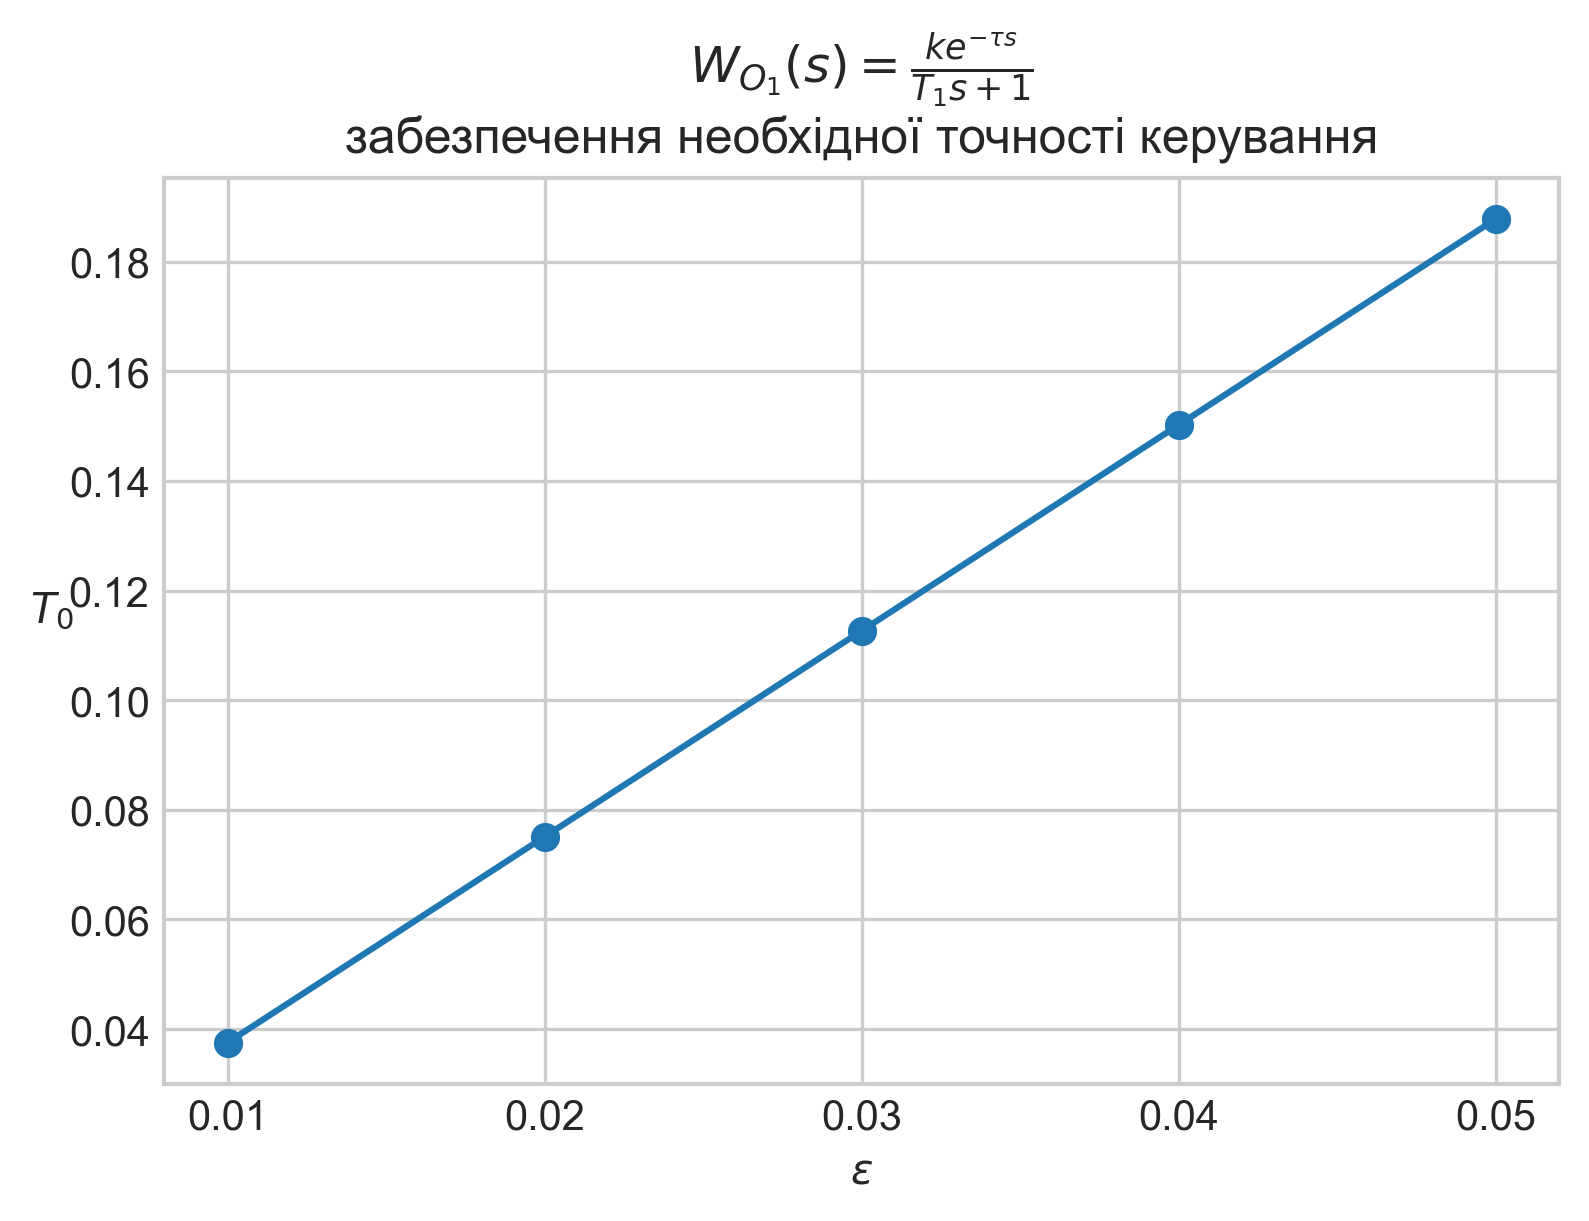
\includegraphics[scale=0.9]{pics/W_01_accur.png}
\end{center}

\subsection{Випадок \texorpdfstring{$W_{O_2}(s) = \frac{k e^{-\tau s}}{(T_1 s + 1)(T_2 s + 1)}$}{2}}
Знайдемо $B(\omega)$:
\begin{gather}
    \mbox{\normalsize $B(\omega) = \omega A(\omega) = \omega \cdot \left| W_{O_2}(j \omega)\right| = 
    \omega \cdot \frac{
        k \left| e^{-\tau j \omega}\right|
    }{
        \left|T_1 j \omega + 1\right| \left|T_2 j \omega + 1\right|
    } = \frac{k \omega}{\sqrt{\left(1 + T_1^2 \omega^2\right)\left(1 + T_2^2 \omega^2\right)}}$}
\end{gather}
$B_{\max}$ можна знайти за допомогою відповідної таблиці:
\begin{gather}
    B_{\max} = \frac{k}{T_1 + T_2} \Rightarrow T_0 = \frac{\varepsilon (T_1 + T_2)}{k}
\end{gather}
Отже, отримуємо наступні періоди квантування для різних $\varepsilon$:
\begin{center}
    \begin{tabular}{|c|c|c|c|c|c|}
        \hline
        $\varepsilon$ & $0.01$ & $0.02$ & $0.03$ & $0.04$ & $0.05$ \\
        \hline
        $T_0$ & $0.0579$ & $0.1159$ & $0.1738$ & $0.2318$ & $0.2897$ \\
        \hline
    \end{tabular}
\end{center}
Залежність $T_0$ від $\varepsilon$:
\begin{center}
    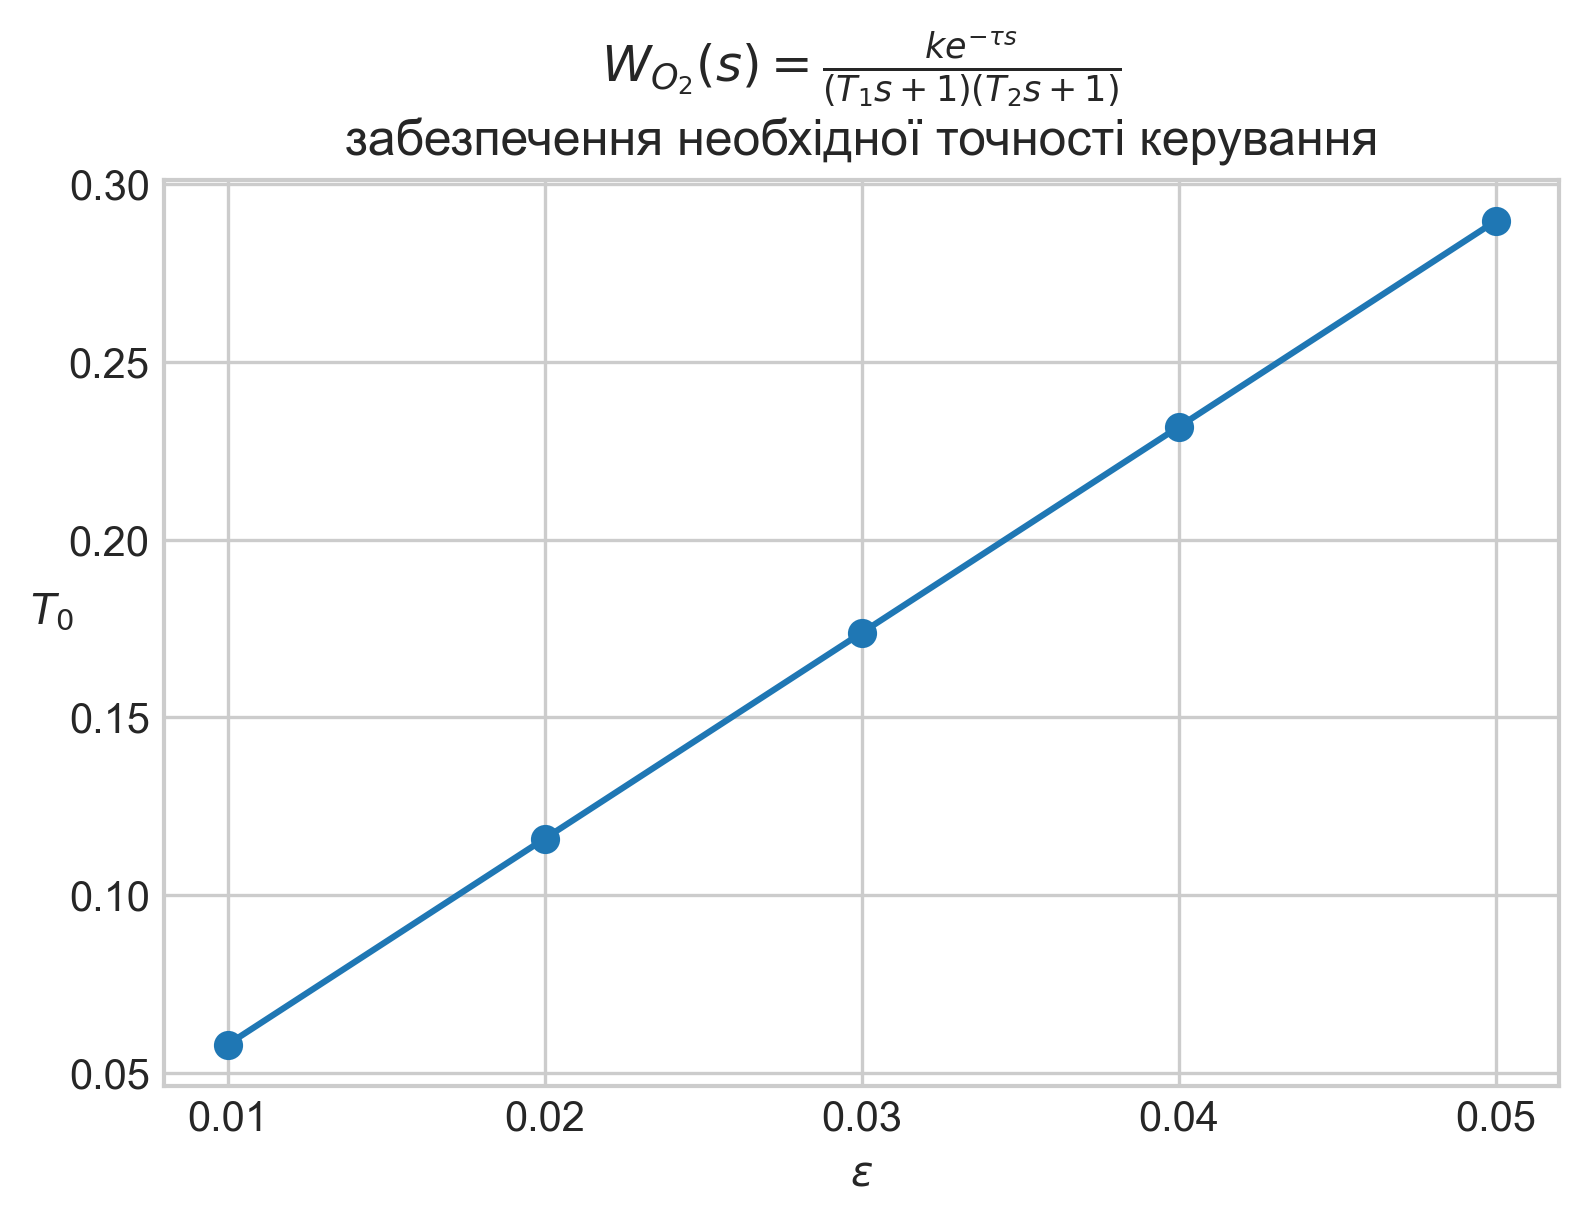
\includegraphics[scale=0.9]{pics/W_02_accur.png}
\end{center}

\section{Розрахунок за критерієм Джурі}
За цим критерієм період квантування обчислюється як $T_0 = \frac{\pi}{\omega_k}$, де 
$\omega_k$ -- розв'язок рівняння
\begin{gather}
    \left| W_{\text{з}}(j\omega_k) \right|
    = \left|
        \frac{W_O (j \omega_k) W_p (j \omega_k)}{
            1 + W_O (j \omega_k) W_p (j \omega_k)
        }
    \right| = \varepsilon
\end{gather}

\subsection{Випадок \texorpdfstring{$W_{O_1}(s) = \frac{k e^{-\tau s}}{T_1 s + 1}$}{1}}
Згідно з розділом \ref{ch:direct}, оптимальним регулятором в цьому випадку є ПІ-регулятор з передаточною функцією 
$W_p(s) = K_p \left(1 + \frac{1}{T_I s}\right) = K_p \cdot \frac{T_1 s + 1}{T_1 s}$, де $K_p = \frac{\lambda T_1}{k \left(1 + \lambda \tau\right)}$, $\lambda = \frac{1}{T_1}$, $T_I = T_1$.
Знайдемо $\left| W_{\text{з}}(j\omega) \right|$:
\begin{gather*}
    \left| W_{\text{з}}(j\omega) \right| = \frac{
        \left| W_{O_1} (j \omega) W_p (j \omega) \right|
    }{
        \left| 1 + W_{O_1} (j \omega) W_p (j \omega) \right|
    } = 
    \frac{
        \left|\frac{k e^{-\tau j \omega}}{T_1 j \omega + 1} \cdot  K_p \cdot \frac{T_1 j \omega + 1}{T_1 j \omega} \right|
    }{
        \left|1 + \frac{k e^{-\tau j \omega}}{T_1 j \omega + 1} \cdot  K_p \cdot \frac{T_1 j \omega + 1}{T_1 j \omega} \right|
    } = \\ =
    \frac{
        \left|k K_p e^{-\tau j \omega} \right|
    }{
        \left|T_1 j \omega + k K_p  e^{-\tau j \omega} \right|
    } = \frac{
        1
    }{
        \left|1 + \frac{T_1}{k K_p} j \omega e^{\tau j \omega} \right|
    } = \frac{
        1
    }{
        \left|1 + \frac{T_1}{k K_p} j \omega \left(\cos \tau\omega + j \sin \tau\omega\right) \right|
    } = \\ =
    \frac{
        1
    }{
        \left| 1 + \frac{T_1}{k K_p}
        \left(j \omega \cos \tau\omega - \omega \sin \tau\omega\right) \right|
    } = \frac{
        1
    }{
        \left| 1 - \frac{T_1}{k K_p} \omega \sin \tau\omega + 
        j \frac{T_1}{k K_p} \omega \cos \tau\omega\right|
    } = \\ = \frac{
        1
    }{
        \sqrt{
            \left(1 - \frac{T_1}{k K_p} \omega \sin \tau\omega\right)^2 +
            \left(\frac{T_1}{k K_p} \omega \cos \tau\omega\right)^2
        }
    } = \frac{
        1
    }{
        \sqrt{
            \left(\frac{T_1}{k K_p}\right)^2 \omega^2 - 2\frac{T_1}{k K_p} \omega \sin \tau\omega + 1
        }
    }
\end{gather*}
Отже, $\left| W_{\text{з}}(j\omega) \right| = \varepsilon \Leftrightarrow \left(\frac{T_1}{k K_p}\right)^2 \omega^2 - 2\frac{T_1}{k K_p} \omega \sin \tau\omega + 1 = \frac{1}{\varepsilon^2}$.
Отримуємо наступні періоди квантування для різних $\varepsilon$:
\begin{center}
    \begin{tabular}{|c|c|c|c|c|c|}
        \hline
        $\varepsilon$ & $0.01$ & $0.02$ & $0.03$ & $0.04$ & $0.05$ \\
        \hline
        $T_0$ & $1.5430$ & $3.0234$ & $4.6304$ & $5.9449$ & $7.9803$ \\
        \hline
    \end{tabular}
\end{center}
Залежність $T_0$ від $\varepsilon$:
\begin{center}
    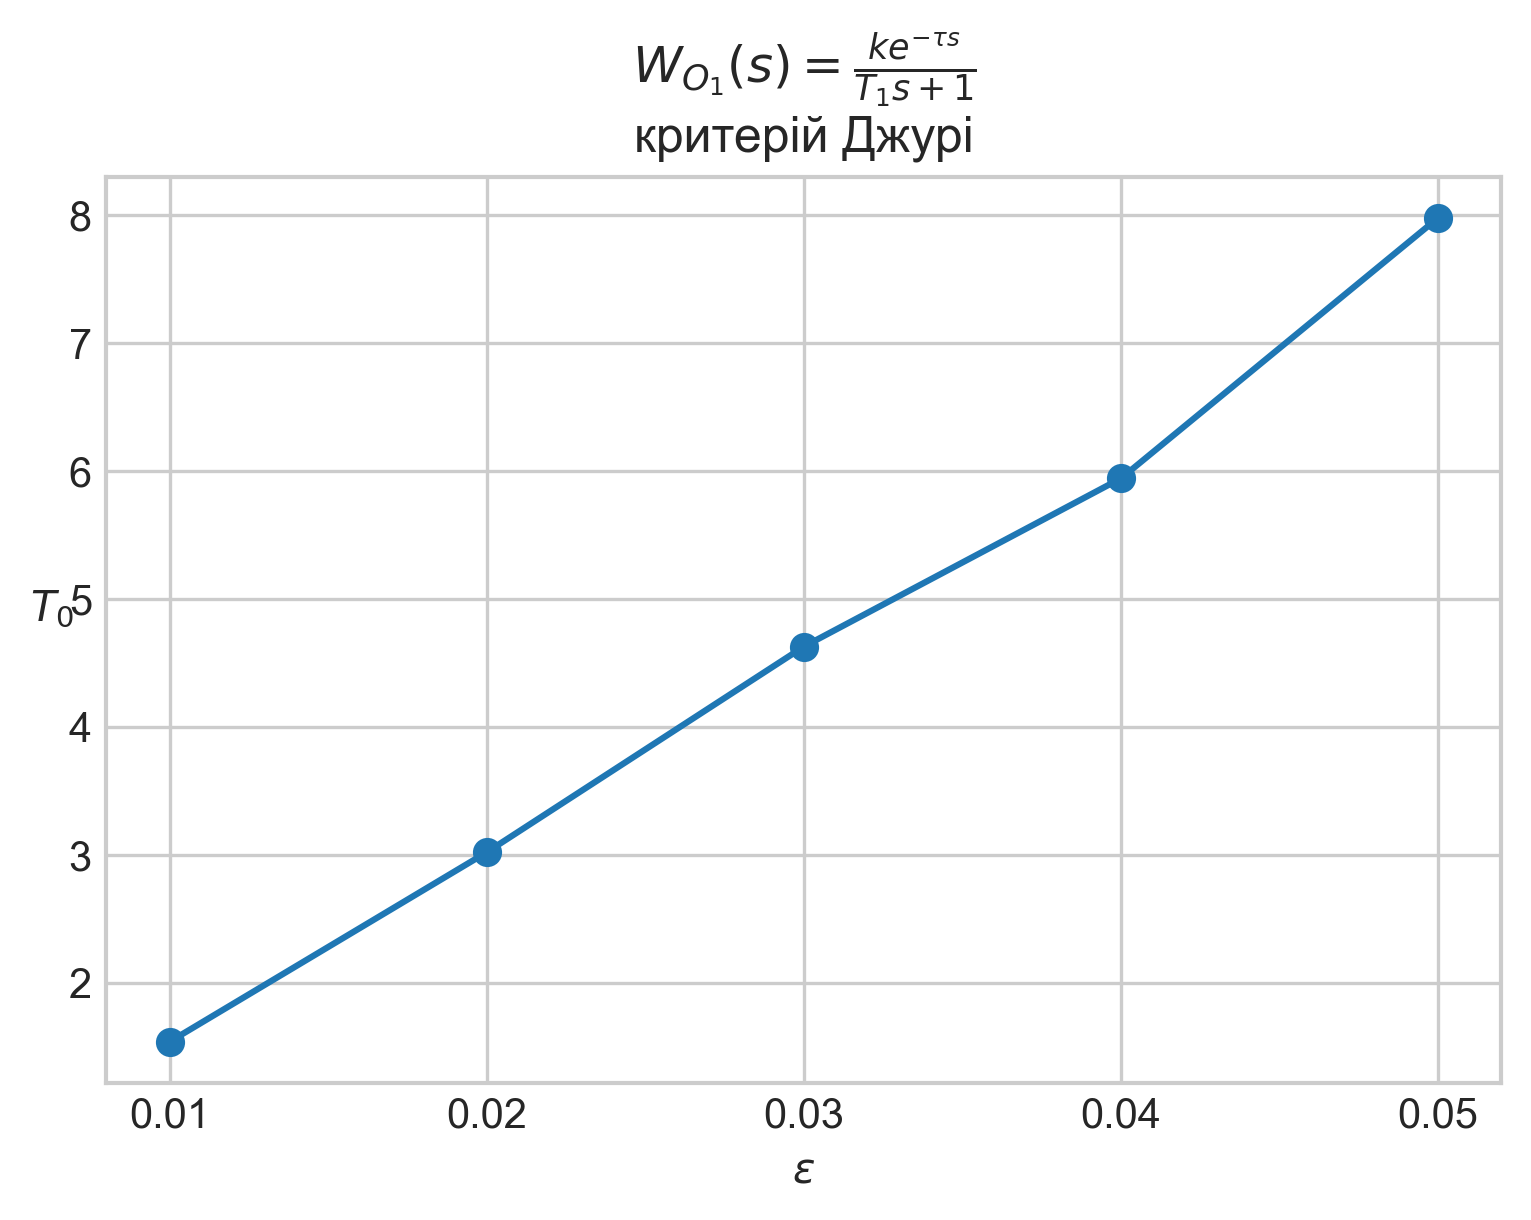
\includegraphics[scale=0.9]{pics/W_01_Jury.png}
\end{center}

\subsection{Випадок \texorpdfstring{$W_{O_2}(s) = \frac{k e^{-\tau s}}{(T_1 s + 1)(T_2 s + 1)}$}{2}}
Згідно з розділом \ref{ch:resonance}, оптимальним регулятором в цьому випадку є ПІ-регулятор з передаточною функцією 
$W_p(s) = K_p \left(1 + \frac{1}{T_I s}\right) = K_p \cdot \frac{T_1 s + 1}{T_1 s}$, де $K_p = ?$, $T_I = ?$.
Знайдемо $\left| W_{\text{з}}(j\omega) \right|$: ???

\section{Розрахунок для об'єкта з динамікою в чисельнику}
Розглядається об'єкт з передаточною функцією $W_O(s) = \frac{
    k (T_1 s + 1)
}{
    (T_2 s + 1) (T_3 s + 1)
}$. Через те, що передаточна функція має динаміку в чисельнику, критерій забезпечення необхідної точності керування
та критерій Джурі непридатні для застосування. Приведемо передаточну функцію до вигляду
$W_O(s) = \frac{K (b T s + 1)}{T^2 s^2 + 2 \nu T s + 1}$:
\begin{gather*}
    \frac{
        k (T_1 s + 1)
    }{
        (T_2 s + 1) (T_3 s + 1)
    } = \frac{k (T_1 s + 1)}{T_2 T_3 s^2 + (T_2 + T_3) s + 1}
\end{gather*}
тому $T = \sqrt{T_2 T_3} \approx 14.4568$, $b = \frac{T_1}{T} \approx 2.421$, $\nu = \frac{T_2 + T_3}{2\sqrt{T_2 T_3}} = \frac{T_2 + T_3}{2T} \approx 1.0376$.
Знайдемо $\left|W_O (j \omega)\right|$:
\begin{gather*}
    \left|W_O (j \omega)\right| = \frac{
        k \left| bT \cdot j \omega + 1 \right|
    }{
        \left| -T^2 \omega^2 + 2\nu T \cdot j \omega + 1\right|
    } = 
    \frac{
        k \sqrt{1 + b^2 T^2 \omega^2}
    }{
        \sqrt{
            \left(1 - T^2 \omega^2\right)^2 + 4 \nu^2 T^2 \omega^2
        }
    }
\end{gather*}
Введемо $\omega_{\text{зр}} = \frac{q}{T}$ -- найвищу частоту сигналу, який необхідно відновити на виході системи:
\begin{gather*}
    \left|W_O (j \omega_{\text{зр}})\right| = 
    \frac{k\sqrt{1 + b^2 q^2}}{
        \sqrt{
            \left(1 - q^2\right)^2 + 4 \nu^2 q^2
        }
    }
\end{gather*}
Розв'яжемо рівняння $\left|W_O (j \omega_{\text{зр}})\right| = \frac{1}{\theta}$, де $\theta = 31$, відносно $q$:
\begin{gather*}
    \frac{k\sqrt{1 + b^2 q^2}}{
        \sqrt{
            \left(1 - q^2\right)^2 + 4 \nu^2 q^2
        }
    } = \frac{1}{\theta} \Leftrightarrow
    \frac{1 + b^2 q^2}{1 - 2 q^2 + q^4 + 4 \nu^2 q^2} = \frac{1}{k^2 \theta^2} \Leftrightarrow \\
    \Leftrightarrow 
    1 - 2 q^2 + q^4 + 4 \nu^2 q^2 = k^2 \theta^2 \left(1 + b^2 q^2\right) \Leftrightarrow \\
    \Leftrightarrow
    q^4 + q^2 \left(4 \nu^2 - b^2 k^2 \theta^2 - 2\right) q^2 + \left(1 - k^2 \theta^2\right) = 0
\end{gather*}
Розв'яжемо це рівняння спочатку відносно $q^2$. Приблизні значення коренів: 
\begin{gather*}
    \left[
        \begin{array}{ll}
            q^2 = 489263.8397 \\
            q^2 = -0.17061
        \end{array}
    \right.
\end{gather*}
Оскільки комплексні та від'ємні $q$ не розглядаються, то отримуємо $q \approx 699.474$.
Отже, період квантування $T_0 = \frac{\pi}{\omega_{\text{зр}}} = 
\frac{\pi T}{q} = 0.0649$.
\end{document}